

\begin{table}[t]
    \centering
    \small
    \begin{tabular}{llc}
    \toprule
    \textbf{Sub-task} & \textbf{DeepSeek-7B} & \textbf{Skywork-7B} \\
    \midrule
    \multicolumn{3}{l}{\textit{Mathematics}} \\
    \quad COMP.en   & 8.61\% $\rightarrow$ 8.46\%  & 4.75\% $\rightarrow$ 7.12\% \\
    \quad COMP.zh   & 7.35\% $\rightarrow$ 7.60\%  & 5.39\% $\rightarrow$ 5.39\% \\
    \quad CEE.zh    & 10.65\% $\rightarrow$ 10.56\% & 8.79\% $\rightarrow$ 9.35\% \\
    \midrule
    \multicolumn{3}{l}{\textit{Physics}} \\
    \quad COMP.en   & 1.69\% $\rightarrow$ 0.00\%  & 0.85\% $\rightarrow$ 1.69\% \\
    \quad CEE.zh    & 7.83\% $\rightarrow$ 11.30\% & 3.48\% $\rightarrow$ 5.22\% \\
    \midrule
    \textbf{Average Acc.}  & \textbf{7.23\% $\rightarrow$ 7.58\%} & \textbf{4.65\% $\rightarrow$ 5.75\%} \\
    \bottomrule
    \end{tabular}
    \caption{\textbf{Performance on OlympiadBench.} Results are shown as Base model $\rightarrow$ KnowRL-trained.}
    \vspace{-3ex}
    \label{tab:olympiadbench_optimized_concise}
\end{table}



\begin{table*}[t]
    \centering
    \footnotesize 
    \setlength{\tabcolsep}{3.0pt} 
    \begin{tabular}{l|cc|cc@{\hskip 10pt}cc|cc@{\hskip 10pt}cc|cc}
    \toprule
    \multirow{3}{*}{\makecell[c]{\textbf{Methods}}} & \multicolumn{10}{c|}{\textbf{Hallucination}} & \multicolumn{2}{c}{\textbf{Reasoning}} \\
    \cmidrule(lr){2-11} \cmidrule(lr){12-13}
    & \multicolumn{2}{c|}{\textbf{TruthfulQA}} & \multicolumn{4}{c|}{\textbf{SimpleQA}} & \multicolumn{4}{c|}{\textbf{ChineseSimpleQA}} & \multirow{2}{*}{\makecell[c]{\small\textbf{GPQA}\\\small\textbf{Diamond}}} & \multirow{2}{*}{\small\textbf{AIME}}\\
    \cmidrule(lr){2-3} \cmidrule(lr){4-7} \cmidrule(lr){8-11}
    & \small\textbf{Rouge} & \small\textbf{Bleu} & \small\textbf{PAQ} & \small\textbf{Incorrect} & \small\textbf{Refusal} & \small\textbf{F1} & \small\textbf{PAQ} & \small\textbf{Incorrect} & \small\textbf{Refusal} & \small\textbf{F1} & & \\
    \midrule
    \rowcolor{lightgray} \multicolumn{13}{c}{\textit{\textbf{Skywork-OR1-7B-Preview}}} \\
    \midrule
    \text{Zero-shot}    & 56.67 & \textbf{55.33} & 2.97 & 76.33 & 21.33 & 2.61 & 11.84 & 67.00 & 24.00 & 10.23 & 37.37 & 26.67  \\
    \text{Self-Refine}   & \underline{58.00} & 54.00 & 3.90 & \perf{74.00}{-2.33} & 23.00 & 3.90 & 9.82 & \perf{67.33}{+0.33} & 25.33 & 8.40 & 46.67 & 36.67 \\
    \text{FactTune-FS}       & \textbf{58.33} & 50.33 & 0.76 & \perf{43.33}{-33.0} & \textbf{56.33} & 0.46 & 8.52 & \perf{68.00}{+1.00} & \underline{25.67} & 7.26 & 40.91 & 26.67  \\
    \text{DPO}                 & 52.67 & 49.33 & \underline{4.81} & \perf{85.66}{+9.33} & 10.00 & \underline{4.56} & \underline{12.64} & \perf{78.33}{+11.3} & 10.33 & \underline{11.95} & 34.85 & 30.00 \\
    \text{SFT}                 & 57.67 & 51.67 & \textbf{11.45} & \perf{77.33}{+1.00} & 12.67& \textbf{10.68} & \textbf{19.70}&\perf{70.67}{+3.67}& 12.00& \textbf{18.44}& 34.85 & 23.33  \\
     \text{TruthRL}              & 57.33 & 50.60 & 3.78 & \perf{56.00}{-20.3} & \underline{41.67} & 2.95 & 10.58 & \perf{62.00}{-5.00} & 30.67 & 8.66 & 39.39 & 26.67 \\
    \text{KnowRL}                & 57.67 & \underline{54.33} & 3.21 & \perf{60.33}{-16.0} & 37.67 & 2.46 & 12.29 & \perf{52.33}{-14.7} & \textbf{40.33} & 9.19 & 42.42 $\uparrow$ & 36.67 $\uparrow$ \\[3pt]
    \midrule
    \rowcolor{lightgray} \multicolumn{13}{c}{\textit{\textbf{DeepSeek-R1-Distill-Qwen-7B}}} \\
    \midrule
    \text{Zero-shot}    & 53.33 & 51.00 & 2.09 & 78.00 & 20.33 & 1.86 & 8.07 & 68.33 & 25.67 & 6.88 & 40.91 & 30.00  \\
    \text{Self-Refine}         & 55.00 & 50.33 & 2.52 & \perf{77.33}{-0.67} & 20.67 & 2.23 & 8.11 & \perf{68.00}{-0.33} & \underline{26.00} & 6.90 & 45.45 & 33.33  \\
    \text{FactTune-FS}         & 54.00 & 50.00 & 2.72 & \perf{59.67}{-18.3} & \underline{38.67} & 2.07 & 10.24 & \perf{76.00}{+7.67} & 15.33 & 9.39 & 38.89 & 30.00  \\
    \text{DPO}                 & 54.00 & 51.00 & \underline{4.35} & \perf{88.00}{+10.0} & 8.00 & \underline{4.16} & \underline{13.14} & \perf{79.33}{+11.0} & 8.67 & \underline{12.54} & 37.37 & 30.00 \\
    \text{SFT}                 & \textbf{57.67} & \underline{52.00} & \textbf{8.42} & \perf{83.33}{+5.33}& 9.00 & \textbf{8.03} & \textbf{19.58} & \perf{76.67}{+8.34}& 4.67& \textbf{19.11} & 36.36 & 26.67  \\
    \text{TruthRL}              & \textbf{57.67} & \textbf{54.67} & 2.14 & \perf{61.00}{-17.0} & 37.67 & 1.64 & 5.76 & \perf{60.00}{-8.33} & \textbf{36.33} & 4.48 & 39.39 & 26.67 \\
    \text{KnowRL}                & \underline{57.33} & 51.60 & 2.81 & \perf{57.67}{-20.3} & \textbf{40.67} & 2.09 & 10.26 & \perf{58.33}{-10.0} & 35.00 & 8.08 & 36.87 $\downarrow$ &  33.33 $\uparrow$ \\
    \bottomrule
    \end{tabular}
    \caption{\textbf{Main Experimental Results.} Performance of KnowRL compared against baselines on the Skywork-OR1-7B-Preview and DeepSeek-R1-Distill-Qwen-7B models. Zero-shot refers to the original model performance. The best results are marked in \textbf{bold}.}
    \vspace{-3ex}
    \label{main-exp}
\end{table*}



\begin{figure*}[t]
    \centering
    \begin{subfigure}[b]{0.32\textwidth}
        \centering
        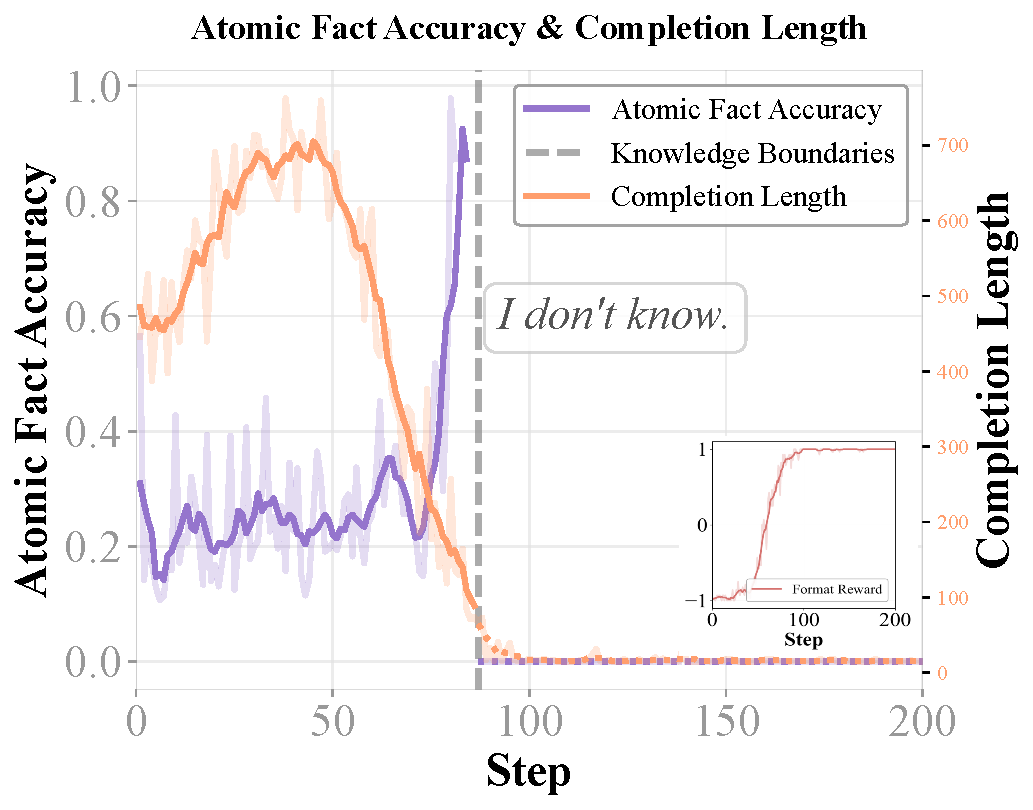
\includegraphics[width=\linewidth]{images/Skywork_final.pdf}
        \caption{The Training Curves (Skywork-OR1-7B-Preview)}
        \label{fig:sub1}
    \end{subfigure}
    \hfill
    \begin{subfigure}[b]{0.32\textwidth}
        \centering
        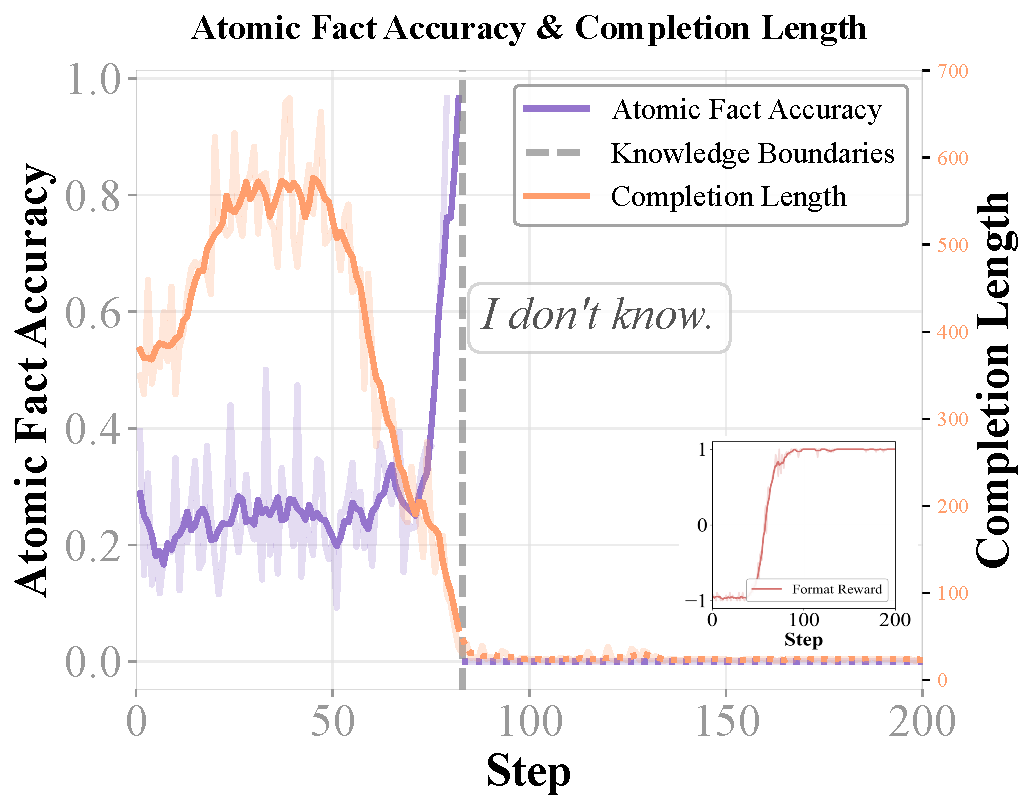
\includegraphics[width=\linewidth]{images/DeepSeek_final.pdf}
        \caption{The Training Curves (DeepSeek-R1-Distill-Qwen-7B)}
        \label{fig:sub2}
    \end{subfigure}
    \hfill
    \begin{subfigure}[b]{0.32\textwidth}
        \centering
        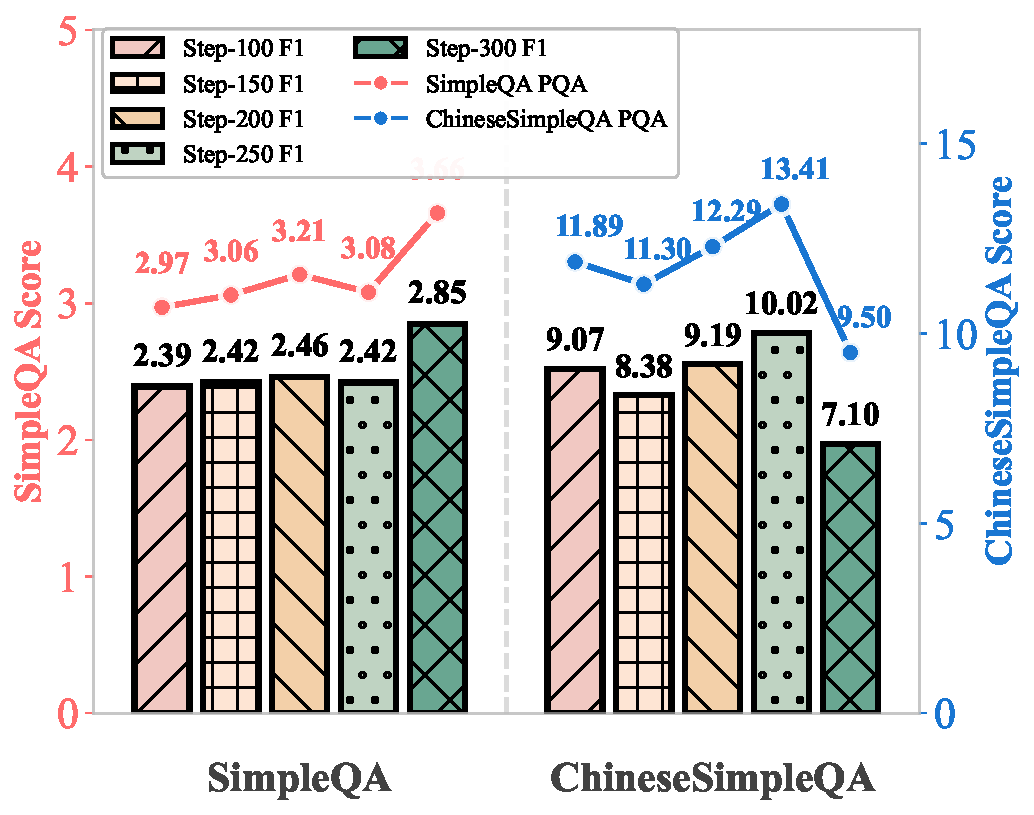
\includegraphics[width=\linewidth]{images/f1_pqa_dual_axis_analysis.pdf}
        \caption{F1 and PAQ Across Training Steps on SimpleQA and ChineseSimpleQA}
        \label{fig:sub3}
    \end{subfigure}
    \hfill
    \begin{subfigure}[b]{0.32\textwidth}
        \centering
        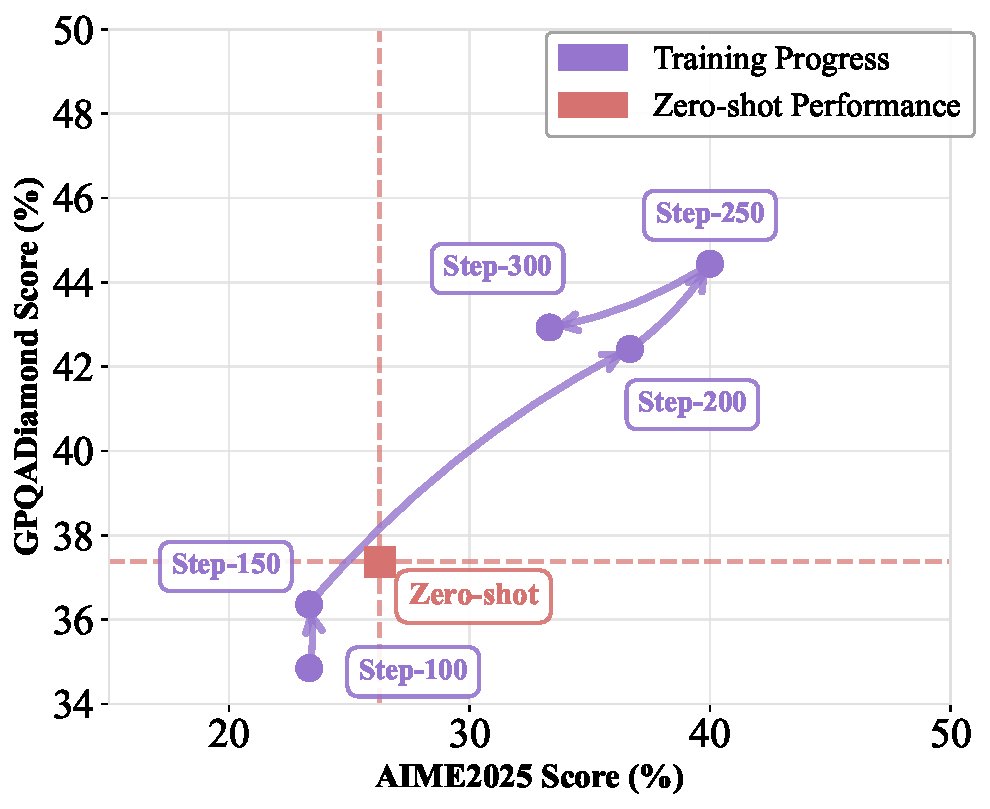
\includegraphics[width=\linewidth]{images/gpqa_aime_analysis.pdf}
        \caption{Training Progress on GPQA and AIME~2025}
        \label{fig:sub4}
    \end{subfigure}
    \hfill
    \begin{subfigure}[b]{0.32\textwidth}
        \centering
        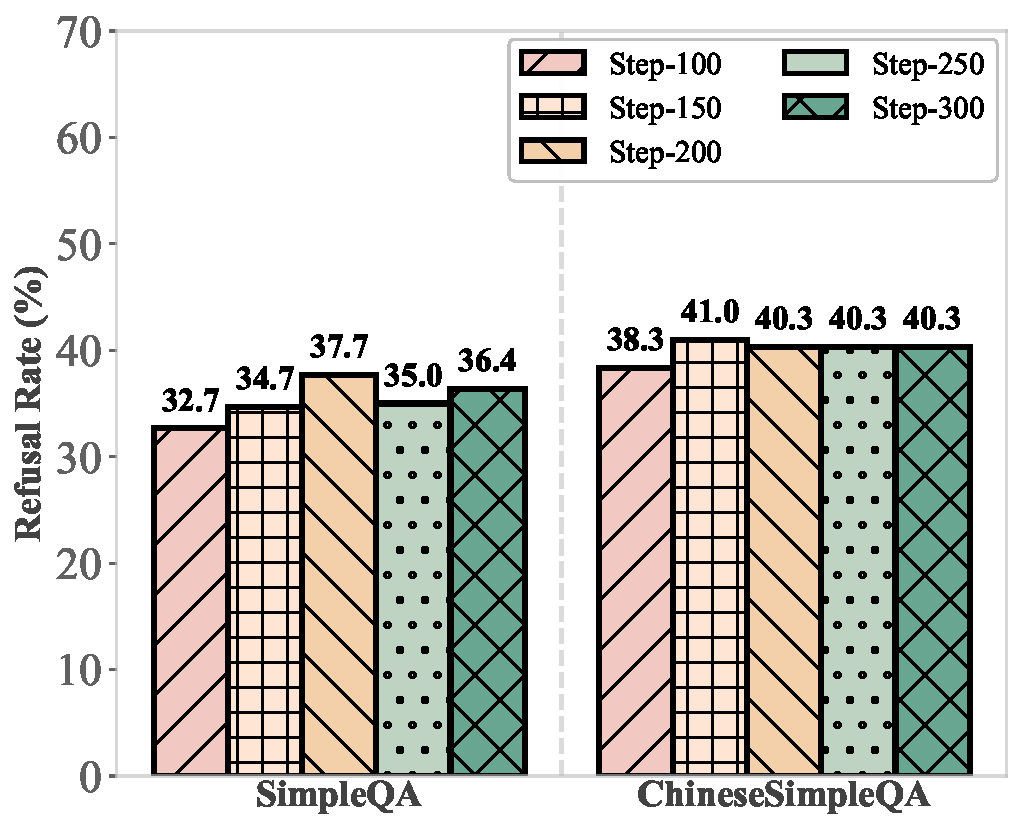
\includegraphics[width=\linewidth]{images/refusal_rates_analysis.pdf}
        \caption{Refusal Rates Across Training Steps on SimpleQA and ChineseSimpleQA}
        \label{fig:sub5}
    \end{subfigure}
    \hfill
    \begin{subfigure}[b]{0.32\textwidth}
        \centering
        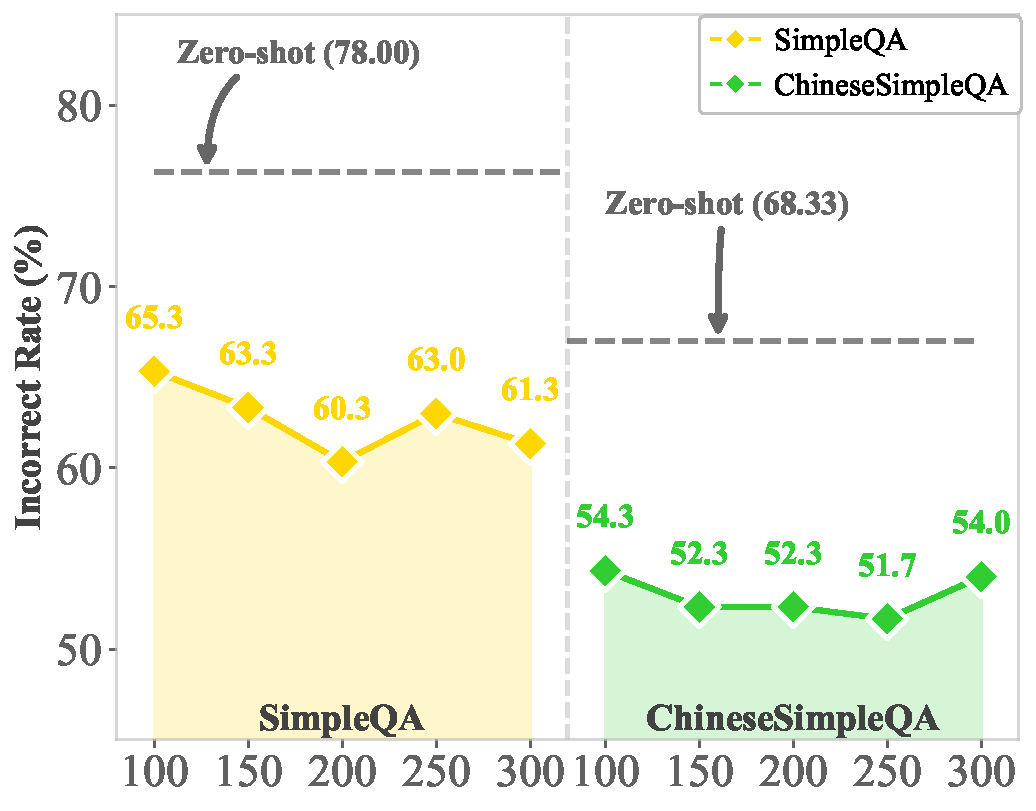
\includegraphics[width=\linewidth]{images/incorrect_rates_baseline_analysis.pdf}
        \caption{Incorrect Rates Across Training Steps vs. Zero-shot Performance}
        \label{fig:sub6}
    \end{subfigure}
    \caption{
    KnowRL training dynamics and reasoning behavior analysis. 
    (a)--(b) present the training curves of two model architectures, showing improved factual alignment and stable reasoning length. 
    (c)--(f) illustrate performance trends of Skywork-OR1-7B-Preview across different training steps, including F1 and PAQ (c), reasoning accuracy (d), refusal rate (e), and incorrect rate (f).
    }
    \vspace{-3ex}
    \label{fig:knowrl-exp}
\end{figure*}



% \begin{table*}[t]
%     \centering
%     \small
%     \setlength{\tabcolsep}{3.2pt}
%     \renewcommand{\arraystretch}{1.2} % Slightly increase row height for readability
%     \begin{tabular}{l|ccc|cc}
%     \toprule
%     \multirow{2}{*}{\makecell[c]{\normalsize\textbf{Reward}}} & \multicolumn{3}{c|}{\textbf{Hallucination}} & \multicolumn{2}{c}{\textbf{Reasoning}} \\
%     \cmidrule(lr){2-4} \cmidrule(lr){5-6}
%     & \small\textbf{TruthfulQA} & \small\textbf{SimpleQA} & \small\textbf{ChineseSimpleQA}  & 
%     \small\textbf{GPQA Diamond} & \small\textbf{AIME 2025}\\
   
%     \midrule
%     \multicolumn{6}{c}{\textbf{DeepSeek-R1-Distill-Qwen-7B}} \\
%     \text{Direct Generation}   & 33.05 & 1.92 & \textbf{11.17}  & 34.34 & 16.67  \\
%     \text{Format}              & 33.41 & \textbf{2.36} & 10.47  & 35.86 & 10.00  \\
%     \text{Format+Fact}         & 34.03 & 1.55 & 9.70  & 31.31 & 16.67  \\
%     \text{Format+Correct}      & \textbf{34.76}  & 1.74 & 10.97 & \textbf{37.88} & \textbf{20.00}  \\
%     \rowcolor{tablehighlight} % Changed color here
%     \text{Format+Fact+Correct} & 33.54 & 1.34 & 11.00 & 34.34 & 6.67  \\
       
%     \midrule
%     \multicolumn{6}{c}{\textbf{DeepSeek-R1-Distill-Qwen-7B-ColdStart}} \\
%     \text{Direct Generation}      & 35.86 & 3.75 & 12.70 & \textbf{39.39} & \textbf{20.00 }  \\
%     \text{Format}                & 36.84 & 3.73 & 14.37 & 35.86 & 16.67  \\
%     \text{Format+Fact}           & 37.82 & \textbf{6.16} & \textbf{14.60} & 35.86 & 13.33 \\
%     \text{Format+Correct}        & 37.82 & 4.04 & 13.80 & 33.33 & 16.67 \\
%     \rowcolor{tablehighlight} % Changed color here
%     \text{Format+Fact+Correct}   & \textbf{38.19} & 4.56 & 13.90 & 37.37 & 13.33 \\
    

%     \bottomrule
%     \end{tabular}
%     \vspace{-1ex}
%     \caption{\textbf{Reward Ablation Experiment.} DeepSeek-R1-Distill-Qwen-7B is trained with cold start to obtain DeepSeek-R1-Distill-Qwen-7B-ColdStart. The best results are marked in \textbf{bold}.}
%     \vspace{-3ex}
%     \label{ablation}
% \end{table*}





\section{Experiments}
\subsection{Experimental Settings.}
\paragraph{Datasets and Metrics.}
We use TruthfulQA~\citep{lin2021truthfulqa}, SimpleQA, and ChineseSimpleQA to evaluate hallucination, and GPQA (general domain) and AIME 2025 (mathematical reasoning) to evaluate reasoning ability.
For the hallucination evaluation datasets, we randomly sample 300 examples from each of TruthfulQA, SimpleQA, and ChineseSimpleQA as test sets.
Because slow-thinking models generate thousands of tokens per query, evaluating full datasets is computationally prohibitive.
A 300-example subset remains highly challenging and provides a statistically valid evaluation, which is a standard practice for long-reasoning tasks.
TruthfulQA is assessed with the ROUGE and BLEU metrics.
For SimpleQA and ChineseSimpleQA, we evaluate performance using four metrics: (1) Incorrect Rate, (2) Refusal Rate, (3) Precision on Answered Questions (PAQ), and (4) $F_1$ score.
PAQ measures the proportion of correctly answered questions among those that the model chooses to answer.
For AIME 2025 and GPQA, we assess reasoning performance based on accuracy metric.
All models are evaluated with the temperature set to 0.


\paragraph{Models and Baselines.}
We select the Skywork-OR1-7B-Preview \citep{skywork-or1-2025} and the DeepSeek-R1-Distill-Qwen-7B for experiments. 
These models represent the two most popular slow thinking training methods: RL, represented by the Skywork-OR1-7B-Preview model, and distillation, represented by the DeepSeek-R1-Distill-Qwen-7B model. 
We select Self-Refine \citep{madaan2023self} as the baseline for prompt engineering, and SFT, DPO, FactTune-FS \citep{tian2023fine} and TruthRL \citep{wei2025truthrl} as the baselines for post-training methods. 
For DPO, we use the distilled DeepSeek-R1 data as the chosen data; for FactTune-FS, the chosen data is composed of the original model's outputs, which are filtered for high factuality using FactScore. 
We use Low-Rank Adaptation \citep[LoRA;][]{hu2022lora} to train all models. Further training details are provided in the Appendix~\ref{appendix:train-set}.

% \paragraph{Training Details.}
% We use Low-Rank Adaptation \citep[LoRA;][]{hu2022lora} to train all models. 
% % For the ColdStart training stage, we train for 4 epochs, with the learning rate set to 1.0e-4 and a batch size of 2. 
% For the reinforcement learning training stage, we train for 200 steps, with the learning rate set to 1.0e-5.  
% More details can be seen in the Appendix. 
% Additionally, we test our method on two new models with distinct architectures, as detailed in the Appendix.


\subsection{Main Results}
\paragraph{KnowRL significantly mitigates hallucination while maintaining reasoning capabilities.}
As shown in Table~\ref{main-exp}, KnowRL consistently improves factual reliability across all datasets. 
For the DeepSeek-R1-Distill-Qwen-7B model, the Incorrect Rate on SimpleQA drops by over 20\% (from 78.00\% to 57.67\%), with similar improvements observed on ChineseSimpleQA. 
Notably, since our training knowledge source is primarily English-based, the consistent gains on ChineseSimpleQA highlight strong cross-lingual transferability, suggesting that KnowRL helps the model internalize a language-agnostic verification behavior rather than merely memorizing language-specific factual patterns.
Importantly, unlike baseline methods that often suffer from catastrophic forgetting, KnowRL preserves strong performance on complex reasoning benchmarks. 
For instance, it improves the GPQA score from 37.37\% to 42.42\% and maintains stability on AIME 2025, demonstrating that factual supervision does not conflict with deep reasoning abilities.
This favorable trade-off can be attributed to KnowRL's process-level design: by rewarding the factual grounding of individual reasoning steps rather than solely adjusting outcome distributions, the model retains its capacity for extended logical deduction while learning to ground each step in verifiable knowledge.
Furthermore, the dramatic drop in completion length (Figure~\ref{fig:knowrl-exp}(a) and (b)) reflects acquired boundary-awareness rather than a collapse of the slow-thinking process.
The model efficiently truncates wasteful hallucinations for unknown facts while preserving extended reasoning chains for complex logical tasks.




\paragraph{Training dynamics demonstrate that the model progressively learns to recognize knowledge boundaries.}
Figure~\ref{fig:knowrl-exp}(a) and (b) illustrates how KnowRL shapes the model's behavior. 
During training, the accuracy of atomic facts within the chain-of-thought steadily increases. 
As the model becomes more precise in its reasoning steps, it learns to distinguish known facts from unknown information. 
Consequently, instead of fabricating answers when uncertain, the model learns to abstain, reflected by a rise in the Refusal Rate and a sharp drop in the Incorrect Rate. 
This confirms that KnowRL effectively teaches the model to reason faithfully rather than merely optimizing for lucky guesses.

% As shown in Table~\ref{main-exp}, KnowRL substantially reduces hallucinations across models and languages. 
% Figure~\ref{fig:knowrl-exp}(a) and (b) further reveal the underlying mechanism. 
% During training, the atomic fact accuracy within the chain-of-thought steadily increases, indicating that the model's reasoning process becomes more grounded in verifiable facts. 
% As factual accuracy improves, the model begins to identify when its knowledge is insufficient and learns to abstain from uncertain statements (e.g., outputting ``I don't know'') rather than fabricating answers. 
% This behavioral change aligns with the quantitative trends in Table~\ref{main-exp}, where a higher atomic fact accuracy corresponds to a lower Incorrect Rate and a higher Refusal Rate.

% Together, these results show that KnowRL instills a fact-grounded reasoning paradigm: the model improves atomic fact correctness, becomes aware of its knowledge boundaries, and substantially reduces hallucinations without compromising reasoning ability on datasets such as GPQA and AIME~2025.






% \paragraph{Distillation-based slow-thinking models exhibit a higher training ceiling compared to slow-thinking models trained by RL.} 
% The training curves in Figure~\ref{knowrl-exp} show DeepSeek-R1-Distill-Qwen-7B model achieving a higher combined reward during KnowRL training, with its output length decreases around 110 steps. 
% In contrast, Skywork-OR1-7B-Preview's reward curve during KnowRL training converges to only approximately -0.4. 
% This indicates better training performance for distillation-based models like DeepSeek-R1-Distill-Qwen-7B. 
% This is further supported by Table~\ref{main-exp}, where the KnowRL-trained DeepSeek-R1-Distill-Qwen-7B outperforms all baselines on three hallucination evaluation datasets, while the KnowRL-trained Skywork-OR1-7B-Preview only exceeds all baselines on the ChineseSimpleQA dataset.

% KnowRL's training effect is less pronounced on the initially RL-trained Skywork-OR1-7B-Preview model compared to the distilled DeepSeek-R1-Distill-Qwen-7B. 
% This suggests that RL-trained models might approach a capability ceiling due to converging to a local optimum during their initial RL process, making further improvement by KnowRL difficult due to search space constraints.
% The findings from Reinforcement Learning with Verifiable Rewards \citep[RLVR;][]{yue2025does} support the conclusion that distilled models possess a higher performance ceiling. 
% This is because, unlike methods that merely improve sampling efficiency by narrowing the reasoning search space, distillation allows models to learn genuinely new knowledge from an unreduced search space, enabling more significant enhancement via subsequent RL. 
% Thus, our method effectively reduces hallucination in distilled models, demonstrating its practical utility, and also confirms that stacked RL training can help mitigate hallucinations.

% \begin{table*}[h]
%     \centering
%     \footnotesize 
%     \setlength{\tabcolsep}{3.0pt} 
%     % --- Using @{...} to add extra space after the 'Incorr.' columns ---
%     \begin{tabular}{l|cc@{\hskip 14pt}cc|cc@{\hskip 14pt}cc|cc}
%     \toprule
%     \multirow{3}{*}{\makecell[c]{\textbf{Reward}\\\textbf{Combination}}} & \multicolumn{8}{c|}{\textbf{Hallucination}} & \multicolumn{2}{c}{\textbf{Reasoning}} \\
%     \cmidrule(lr){2-9} \cmidrule(lr){10-11}
%     & \multicolumn{4}{c|}{\textbf{SimpleQA}} & \multicolumn{4}{c|}{\textbf{ChineseSimpleQA}} & \multirow{2}{*}{\makecell[c]{\small\textbf{GPQA}\\\small\textbf{Diamond}}} & \multirow{2}{*}{\small\textbf{AIME}}\\
%     \cmidrule(lr){2-5} \cmidrule(lr){6-9}
%     & \small\textbf{PAQ} & \small\textbf{Incorrect} & \small\textbf{Refusal} & \small\textbf{F1} & \small\textbf{PAQ} & \small\textbf{Incorrect} & \small\textbf{Refusal} & \small\textbf{F1} & & \\
    
%     \midrule
%     \rowcolor{lightgray} \multicolumn{11}{c}{\textit{\textbf{DeepSeek-R1-Distill-Qwen-7B}}} \\
%     \midrule
%     $R = r_{\text{format}}$ & 2.63 & 74.00 & 24.00 & \underline{2.27} & 7.08 & 74.33 & 20.00 & 6.29 & \underline{39.39} & 30.00  \\
%     $R = r_{\text{format}} + r_{\text{fact}}$ & 2.42 & \perf{80.67}{+6.67} & 17.33 & 2.19 & 8.87 & \perf{75.33}{+1.00} & 17.33 & \underline{8.03} & \textbf{47.47} & \textbf{40.00} \\
%     $R = r_{\text{format}} + r_{\text{correct}}$ & \textbf{3.19} & \perf{60.67}{-13.3} & \underline{37.33} & \textbf{2.46} & \underline{8.89} & \perf{41.00}{-33.3} & \textbf{55.00} & 5.52 & 38.89 & \textbf{40.00} \\
%     $R = R_{total}$ (\textbf{KnowRL}) & \underline{2.81} & \perf{57.67}{-16.3} & \textbf{40.67} & 2.09 & \textbf{10.26} & \perf{58.33}{-16.0} & \underline{35.00} & \textbf{8.08} & 37.37 & \underline{33.33} \\
%     \addlinespace[0.5pt] % Adjust the space here
%     KnowRL ($R_{refusal}=-1$) & 1.26 & \perf{78.67}{+4.67} & 20.33 & 1.11 & 7.66 & \perf{84.33}{+10.0} & 8.67 & 7.32 & 34.85 & 30.00 \\
    
%     \bottomrule
%     \end{tabular}
%     \caption{\textbf{Ablation Study.} Ablation study on different reward combinations for the DeepSeek-R1-Distill-Qwen-7B model. The best results are marked in \textbf{bold}, and the second-best results are \underline{underlined}.}
%     \vspace{-3ex}
%     \label{tab:ablation}
% \end{table*}

%$R_{correct}(o=refusal)=-1$




\begin{table*}[h]
    \centering
    \footnotesize 
    \setlength{\tabcolsep}{3.0pt} 
    % --- Using @{...} to add extra space after the 'Incorr.' columns ---
    \begin{tabular}{l|cc@{\hskip 14pt}cc|cc@{\hskip 14pt}cc|cc}
    \toprule
    \multirow{3}{*}{\makecell[c]{\textbf{Method}}} & \multicolumn{8}{c|}{\textbf{Hallucination}} & \multicolumn{2}{c}{\textbf{Reasoning}} \\
    \cmidrule(lr){2-9} \cmidrule(lr){10-11}
    & \multicolumn{4}{c|}{\textbf{SimpleQA}} & \multicolumn{4}{c|}{\textbf{ChineseSimpleQA}} & \multirow{2}{*}{\makecell[c]{\small\textbf{GPQA}\\\small\textbf{Diamond}}} & \multirow{2}{*}{\small\textbf{AIME}}\\
    \cmidrule(lr){2-5} \cmidrule(lr){6-9}
    & \small\textbf{PAQ} & \small\textbf{Incorrect} & \small\textbf{Refusal} & \small\textbf{F1} & \small\textbf{PAQ} & \small\textbf{Incorrect} & \small\textbf{Refusal} & \small\textbf{F1} & & \\
    
    \midrule
    \rowcolor{lightgray} \multicolumn{11}{c}{\textit{\textbf{Ablation on Reward Combination (Base Model: DeepSeek-R1-Distill-Qwen-7B)}}} \\
    \midrule
    $R = r_{\text{format}}$ & 2.63 & 74.00 & 24.00 & \underline{2.27} & 7.08 & 74.33 & 20.00 & 6.29 & \underline{39.39} & 30.00  \\
    $R = r_{\text{format}} + r_{\text{fact}}$ & 2.42 & \perf{80.67}{+6.67} & 17.33 & 2.19 & 8.87 & \perf{75.33}{+1.00} & 17.33 & \underline{8.03} & \textbf{47.47} & \textbf{40.00} \\
    $R = r_{\text{format}} + r_{\text{correct}}$ & \textbf{3.19} & \perf{60.67}{-13.33} & \underline{37.33} & \textbf{2.46} & \underline{8.89} & \perf{41.00}{-33.33} & \textbf{55.00} & 5.52 & 38.89 & \textbf{40.00} \\
    $R = R_{total}$ (KnowRL) & \underline{2.81} & \perf{57.67}{-16.33} & \textbf{40.67} & 2.09 & \textbf{10.26} & \perf{58.33}{-16.00} & \underline{35.00} & \textbf{8.08} & 36.87 & \underline{33.33} \\
    \addlinespace[0.5pt] % Adjust the space here
    KnowRL ($R_{refusal}=-1$) & 1.26 & \perf{78.67}{+4.67} & 20.33 & 1.11 & 7.66 & \perf{84.33}{+10.00} & 8.67 & 7.32 & 34.85 & 30.00 \\
    
    \addlinespace[2pt]
    \midrule
    \rowcolor{lightgray} \multicolumn{11}{c}{\textit{\textbf{Robustness Analysis (Using GRPO reward, $R = R_{total}$)}}}\\
    \midrule
    
    Zero-shot & 2.09 & 78.00 & 20.33 & 1.86 & 8.07 & 68.33 & 25.67 & 6.88 & 40.91 & 30.00 \\
    \addlinespace[0.5pt]
    KnowRL (DAPO) & 1.11 & \perf{59.33}{-18.67} & 40.00 & 0.83 & 9.14 & \perf{59.67}{-8.66} & 34.33 & 7.24 & 41.41 & 43.33 \\
    KnowRL (BNPO) & 1.61 & \perf{61.00}{-17.00} & 38.00 & 1.23 & 11.48 & \perf{61.67}{-6.66} & 30.33 & 9.43 & 41.41 & 30.00 \\
    KnowRL (Dr.GRPO) & 3.16 & \perf{61.33}{-16.67} & 36.67 & 2.45 & 11.33 & \perf{60.00}{-8.33} & 32.33 & 9.15 & 38.38 & 43.33 \\

    \bottomrule
    \end{tabular}
    \caption{\textbf{Ablation and Robustness Analysis.} Impact of reward components and different RL algorithms for the DeepSeek-R1-Distill-Qwen-7B. In reward ablation section, best results are in \textbf{bold} and second-best are \underline{underlined}.}
    \vspace{-3ex}
    \label{tab:ablation}
\end{table*}





















\subsection{Extended Evaluation on Reasoning Benchmarks}
We further evaluate KnowRL on OlympiadBench~\citep{he2024olympiadbench} to examine its impact on complex reasoning in mathematics and physics. 
As shown in Table~\ref{tab:olympiadbench_optimized_concise}, both models maintain or improve their performance after KnowRL training. 
Specifically, the DeepSeek model increases its average accuracy from 7.23\% to 7.58\%, while the Skywork model improves from 4.65\% to 5.75\%. 
Both models achieved significant gains in the Chinese physics task (\textit{physics\_zh\_CEE}), with DeepSeek-7B rising from 7.83\% to 11.30\%. 
Although there are minor fluctuations in individual sub-tasks, the overall trend confirms that factual supervision does not hinder structured reasoning.


Combined with the consistent results on GPQA and AIME~2025, these findings provide strong evidence that \textbf{KnowRL effectively preserves and enhances complex reasoning capabilities across diverse other domains, enabling models to reason more reliably under factual constraints}.





\subsection{Training Step Analysis}
To investigate how the number of KnowRL training steps affects the trade-off between factuality and reasoning, we evaluate models trained for 100, 150, 200, 250, and 300 reinforcement learning steps. 
The results are illustrated in Figure~\ref{fig:knowrl-exp}(c)--(f).

As shown in Figure~\ref{fig:knowrl-exp}(c), both F1 and PAQ scores improve rapidly in the early stage of training and reach a stable high level after moderate training, suggesting that factual precision and reliability are primarily acquired in the middle phase of optimization. 
Reasoning performance on GPQA and AIME~2025 (Figure~\ref{fig:knowrl-exp}(d)) remains stable or slightly improves within this range, indicating that factual supervision can refine reasoning without inducing degradation. 
Refusal rates (Figure~\ref{fig:knowrl-exp}(e)) increase and then plateau, reflecting that models progressively learn appropriate abstention behavior, while the incorrect rate (Figure~\ref{fig:knowrl-exp}(f)) decreases sharply in early training and stabilizes thereafter. 
Beyond this stage, additional optimization provides limited factual improvement and introduces minor task-dependent variations rather than consistent gains.

These observations suggest that KnowRL’s reinforcement learning dynamics follow a stable convergence pattern rather than the reversal effects sometimes observed in overfitted reasoning models~\citep{berglund2023reversal}. 
Appropriate training duration is therefore crucial: insufficient updates hinder factual learning, whereas excessive optimization may overfit factual supervision signals and weaken generalization.

\textbf{Overall, KnowRL achieves its best balance between factuality and reasoning stability when trained for an appropriate number of reinforcement learning steps, where the model fully internalizes factual supervision without over-optimization or reasoning drift.}


\subsection{Ablation Study}

%\subsection{Impact of Reward Components}

To understand how different reward signals contribute to the model's performance, we evaluate the DeepSeek-R1-Distill-Qwen-7B model under different reward combinations.

\paragraph{Factual reward ($r_{fact}$) enhances fact-grounded reasoning.}
As shown in Table~\ref{tab:ablation}, using the factual reward alone achieves the best performance on reasoning benchmarks such as GPQA and AIME~2025. 
This shows that $r_{\text{fact}}$ encourages models to perform reasoning grounded in verifiable knowledge, helping them maintain accuracy while reducing random errors. 
This finding underscores the importance of factual verification in the reinforcement learning process, consistent with prior work showing that incorporating verifiable rewards can substantially improve the reliability and stability of RL training~\citep[RLVR;][]{yue2025does}.


\paragraph{Positive refusal incentives promote boundary awareness.} Table~\ref{tab:ablation} shows that giving a positive reward for refusals leads to higher refusal rates and fewer hallucination errors. 
This explicitly encourages the model to admit when it lacks knowledge.
When we removed this positive incentive (setting $R_{\text{refusal}}=-1$), the incorrect rate increased significantly.
This confirms that rewarding appropriate refusals is essential for learning knowledge boundaries.

% \paragraph{Correct reward ($r_{\text{correct}}$) with positive refusal incentives promotes boundary awareness.}
% Table~\ref{tab:ablation} shows that the positive reward assigned to refusals in $r_{\text{correct}}$ leads to higher refusal rates and lower hallucination errors, indicating that such design explicitly encourages the model to recognize when it lacks sufficient knowledge and to abstain from unreliable responses. 
% To further verify that the refusal reward is the key factor driving boundary awareness, we set $R_{\text{correct}}(o \in \text{refusal}) = -1$ in KnowRL and obtain the results of KnowRL ($R_{\text{refusal}}=-1$). 
% As shown in Table~\ref{tab:ablation}, the incorrect rate rises substantially under this setting, confirming that rewarding appropriate refusals is essential for stimulating boundary learning and mitigating hallucinations. 
% This finding aligns with recent analyses of reward shaping for truthful generation~\citep{shao2025spurious}, which emphasize that correctly incentivizing uncertainty recognition is critical for enhancing factual reliability in reinforcement learning–based language models.



% \paragraph{Simple reward combinations are insufficient for mitigating hallucination in factual tasks.} 
% As demonstrated in Table~\ref{ablation}, using simple reward combinations, for example 'Format' and 'Correct' rewards, can even decrease the performance of the DeepSeek-R1-Distill-Qwen-7B on the SimpleQA dataset. 
% This suggests that for open-domain factual tasks, a model can learn to generate answers that satisfy the correctness reward without adhering to a factual reasoning process. Our finding presents a notable contrast to observations in other domains like mathematical reasoning. There, some research suggests that simpler reward combinations can yield performance gains, even if by capitalizing on spurious signals \citep{shao2025spurious}. 
% We, therefore, conclude that for the complex challenge of mitigating hallucinations, a simple combination of rewards is not a reliable solution, underscoring the need for a more comprehensive approach like the full KnowRL framework.

\section{Analysis}

\subsection{Robustness Analysis of Different RL Algorithms}

To verify that the effectiveness of KnowRL is not limited to a specific optimization method, we extended our framework to three additional RL algorithms: BNPO \cite{xiao2025bnpo}, DAPO \citep{yu2025dapo}, and Dr.GRPO \citep{liu2025understanding}. 
We compare their performance using the DeepSeek-R1-Distill-Qwen-7B model.

\paragraph{KnowRL is robust across different algorithms.} 
Table~\ref{tab:ablation} demonstrates that every algorithm achieved the dual goal of our framework: they all significantly reduced the Incorrect Rate compared to the Zero-shot baseline, while successfully maintaining or even improving reasoning performance. 
This confirms that the KnowRL framework effectively reduces hallucinations without compromising reasoning capabilities, regardless of the specific RL algorithm used. 
Detailed analysis of response length and atomic fact accuracy during training is provided in Appendix~\ref{appendix:RL_algorithms}.







\subsection{Analysis of Factors Affecting Knowledge Boundaries}

To examine whether the positive refusal reward in $r_{\text{correct}}$ is the only factor driving boundary learning, we conducted an experiment on the DeepSeek-R1-Distill-Qwen-7B model using SimpleQA and ChineseSimpleQA. 
We modified the KnowRL setting by changing the refusal reward from positive to negative $r_{\text{refusal}=-1}$, while keeping other rewards unchanged. 
We evaluated the model at training steps 0, 100, 150, 200, and 250.

As shown in Figure~\ref{fig:boundary-analysis}, the refusal rate initially rises even without a positive refusal reward. 

This confirms that the positive refusal reward is not the only factor affecting knowledge boundaries; the penalty for incorrect answers also encourages the model to be cautious in the early stages. 
However, this behavior is unstable. 
Later stages in Figure~\ref{fig:boundary-analysis} show a significant drop in refusal rates accompanied by a spike in incorrect answers. 
This occurs because the model learns to guess to maximize scores rather than accepting refusal penalties—known as reward hacking. Thus, while correctness rewards trigger initial caution, positive refusal rewards are essential to maintain it and prevent guessing.
\textbf{Overall, the results suggest that positive refusal rewards are not the only source of boundary learning; 
different reward combinations can jointly promote boundary-aware reasoning.}



We further investigate the scalability and evaluator sensitivity of our framework. 
Experiments on the larger DeepSeek-R1-Distill-Qwen-14B model show that KnowRL consistently reduces hallucinations while improving reasoning capabilities, confirming its scalability across model sizes(details in Appendix~\ref{appendix:scalability}). 
Moreover, we conduct an Evaluator Sensitivity Analysis by replacing the GPT-4o-mini used during training with different model. 
The results indicate that KnowRL maintains robust performance regardless of the specific evaluator used. Comprehensive results for these analyses are provided in Appendix~\ref{appendix:sensitivity}.


\begin{figure}[t]
    \centering
    \resizebox{.41\textwidth}{!}{
    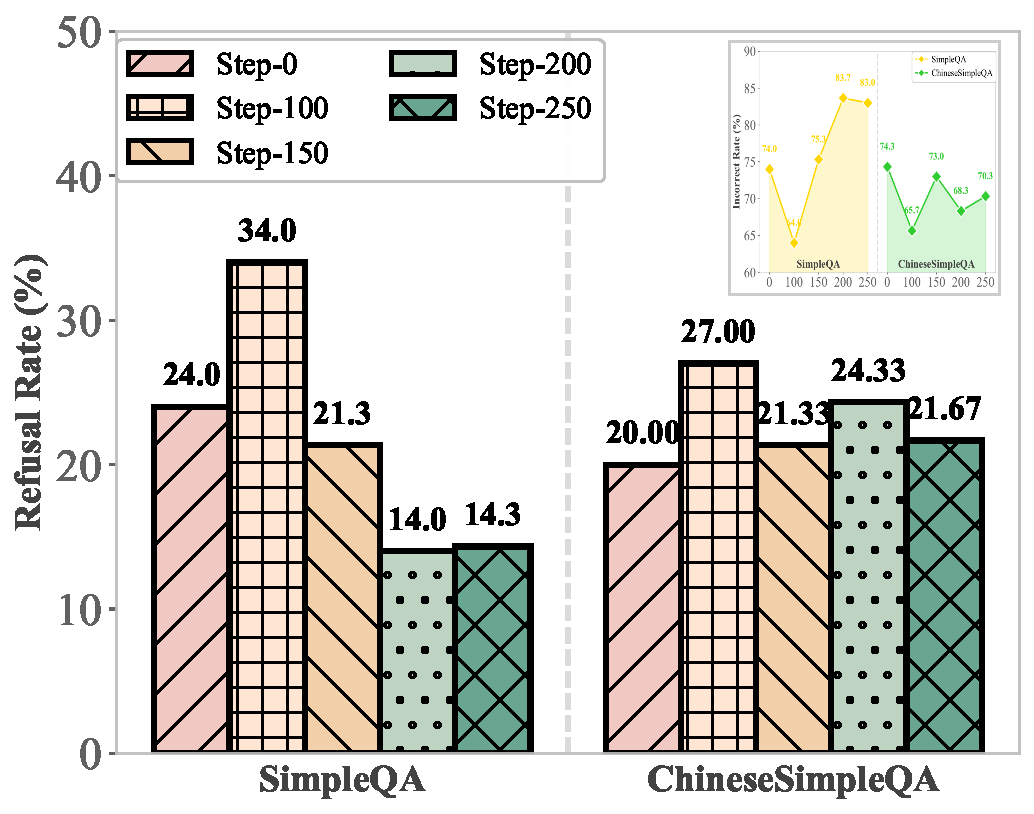
\includegraphics{images/refusal_rates_analysis_with_inset.pdf}}
    \caption{
    Trends of refusal and incorrect rates on SimpleQA and ChineseSimpleQA 
    when training with the combination of format reward and negative refusal reward across different training steps.}
    \vspace{-3ex}
    \label{fig:boundary-analysis}
\end{figure}






\section{Robustness and Multi-run Evaluation}
\label{app:multi_run}

To address the potential sensitivity of single-run evaluations at zero temperature, especially on small-scale benchmarks like AIME, we conduct a robust multi-run evaluation.
We re-evaluate the base models and KnowRL using a non-zero temperature of 0.6, generating 5 responses per prompt to report the average performance (Avg@5).
This setup ensures that the observed improvements in factuality and reasoning are consistent and not artifacts of decoding variance.

\begin{table*}[t]
    \centering
    \footnotesize 
    \setlength{\tabcolsep}{3.0pt} 
    \begin{tabular}{l|cc|cc@{\hskip 10pt}cc|cc@{\hskip 10pt}cc|cc}
    \toprule
    \multirow{3}{*}{\makecell[c]{\textbf{Methods}}} & \multicolumn{10}{c|}{\textbf{Hallucination}} & \multicolumn{2}{c}{\textbf{Reasoning}} \\
    \cmidrule(lr){2-11} \cmidrule(lr){12-13}
    & \multicolumn{2}{c|}{\textbf{TruthfulQA}} & \multicolumn{4}{c|}{\textbf{SimpleQA}} & \multicolumn{4}{c|}{\textbf{ChineseSimpleQA}} & \multirow{2}{*}{\makecell[c]{\small\textbf{GPQA}\\\small\textbf{Diamond}}} & \multirow{2}{*}{\small\textbf{AIME}}\\
    \cmidrule(lr){2-3} \cmidrule(lr){4-7} \cmidrule(lr){8-11}
    & \small\textbf{Rouge} & \small\textbf{Bleu} & \small\textbf{PAQ} & \small\textbf{Incorrect} & \small\textbf{Refusal} & \small\textbf{F1} & \small\textbf{PAQ} & \small\textbf{Incorrect} & \small\textbf{Refusal} & \small\textbf{F1} & & \\
    \midrule
    \rowcolor{lightgray} \multicolumn{13}{c}{\textit{\textbf{Skywork-OR1-7B-Preview}}} \\
    \midrule
    \text{Zero-shot}    & 56.20 & 51.60 & 7.48 & 59.47 & 35.73 & 9.16 & 10.95 & 57.87 & 35.00 & 13.30 & 44.95 & 34.67  \\
    \text{DPO}          & 56.13 & 51.33 & 6.65 & \perf{81.27}{+21.80} & 12.93 & 10.93 & 11.83 & \perf{77.47}{+19.60} & 12.13 & 18.81 & 44.34 & 34.67 \\
    \text{FactTune-FS}  & 57.60 & 53.00 & 3.51 & \perf{44.33}{-15.14} & 54.07 & 2.20 & 10.84 & \perf{40.60}{-17.27} & 54.47 & 9.40 & 45.45 & 34.67  \\
    \text{SFT}          & 57.27 & 50.93 & 9.52 & \perf{61.07}{+1.60} & 32.40 & 10.71 & 8.21 & \perf{78.93}{+21.06} & 14.00 & 7.59 & 39.39 & 38.67  \\
    \text{TruthRL}      & 57.67 & 53.47 & 8.15 & \perf{49.07}{-10.40} & 46.60 & 8.30 & 12.33 & \perf{32.60}{-25.27} & 62.80 & 8.78 & 46.36 & 33.33 \\
    \text{KnowRL}       & 58.27 & 52.80 & 7.32 & \perf{40.20}{-19.27} & \textbf{56.60} & 6.17 & 10.30 & \perf{28.40}{-29.47} & \textbf{68.33} & 6.32 & \textbf{48.89} $\uparrow$ & \textbf{38.00} $\uparrow$ \\[3pt]
    \midrule
    \rowcolor{lightgray} \multicolumn{13}{c}{\textit{\textbf{DeepSeek-R1-Distill-Qwen-7B}}} \\
    \midrule
    \text{Zero-shot}    & 57.40 & 51.53 & 4.89 & 62.47 & 34.33 & 6.20 & 10.23 & 60.27 & 32.93 & 11.83 & 45.45 & 29.33  \\
    \text{DPO}          & 55.60 & 51.40 & 5.65 & \perf{76.33}{+13.86} & 19.07 & 8.74 & 9.54 & \perf{67.20}{+6.93} & 25.73 & 13.20 & 40.40 & 28.67 \\
    \text{FactTune-FS}  & 56.93 & 52.13 & 2.73 & \perf{61.73}{-0.74} & 36.53 & 2.12 & 8.90 & \perf{56.60}{-3.67} & 37.87 & 10.48 & 43.74 & 30.67  \\
    \text{SFT}          & 57.13 & 51.27 & 9.38 & \perf{82.47}{+20.00} & 9.00 & 15.72 & 9.86 & \perf{82.07}{+21.80} & 8.93 & 9.41 & 38.28 & 35.33  \\
    \text{TruthRL}      & 56.27 & 51.94 & 5.93 & \perf{50.73}{-11.74} & 46.07 & 6.19 & 9.37 & \perf{30.47}{-29.80} & 66.40 & 4.69 & 44.34 & 31.33 \\
    \text{KnowRL}       & 57.20 & 52.40 & 5.50 & \perf{48.27}{-14.20} & \textbf{48.93} & 5.43 & 8.38 & \perf{28.07}{-32.20} & \textbf{69.40} & 4.94 & \textbf{46.97} $\uparrow$ & \textbf{34.00} $\uparrow$ \\
    \bottomrule
    \end{tabular}
    \caption{\textbf{Multi-run Evaluation Results.} Robust multi-run performance (Avg@5, Temperature=0.6) of KnowRL compared against baselines on the Skywork-OR1-7B-Preview and DeepSeek-R1-Distill-Qwen-7B models. Zero-shot refers to the original model performance. The key improvements are marked in \textbf{bold}.}
    \vspace{-3ex}
    \label{tab:multi_run_results}
\end{table*}

As shown in Table \ref{tab:multi_run_results}, the multi-run averages consistently support our primary findings.
Even under stochastic decoding, KnowRL significantly improves refusal rates on hallucination-prone queries (SimpleQA and ChineseSimpleQA) while simultaneously enhancing or maintaining performance on complex reasoning tasks (GPQA and AIME).
For instance, KnowRL improves AIME accuracy from 29.33\% to 34.00\% for DeepSeek-7B, confirming that our framework effectively promotes reliable reasoning rather than simply collapsing to conservative refusals.















% \begin{table*}[!htbp]
%     \centering
%     \small
%     \setlength{\tabcolsep}{3.2pt}
%     \renewcommand{\arraystretch}{1.2} % Slightly increase row height for readability
%     \begin{tabular}{l|ccc|cc}
%     \toprule
%     \multirow{2}{*}{\makecell[c]{\normalsize\textbf{KnowRL}}} & \multicolumn{3}{c|}{\textbf{Hallucination}} & \multicolumn{2}{c}{\textbf{Reasoning}} \\
%     \cmidrule(lr){2-4} \cmidrule(lr){5-6}
%     & \small\textbf{TruthfulQA} & \small\textbf{SimpleQA} & \small\textbf{ChineseSimpleQA}  & 
%     \small\textbf{GPQA} & \small\textbf{AIME 2025}\\
   
%     \midrule
%     \multicolumn{6}{c}{\textbf{Skywork-OR1-7B-Preview}} \\
%    \text{Direct Generation}     & 34.39 & 4.58 & 13.27  & 31.31 & 6.67  \\
%    % \text{SFT (ColdStart)}     & 35.99 & 5.14 & 14.67 & 33.84 & 20.00   \\
%     \text{KnowRL Step100}        & 37.45 & 4.31 & 16.37 & 35.86 & 20.00 \\
%     \text{KnowRL Step150}        & 37.70 & 5.04 & 16.23 & 34.34 & 10.00 \\
%     \text{KnowRL Step200}        & 36.96 & 4.82 & 15.33 & 34.34 & 10.00  \\
       
%     % \midrule
%     % \multicolumn{6}{c}{\textbf{DeepSeek-R1-Distill-Qwen-7B}} \\
%     % \text{Direct Generation}     & 33.05 & 1.92 & 11.17  & 34.34 & 16.67  \\
%     % \text{KnowRL Step100}        & 33.17 & 1.25 & 11.17 & 34.34 & 13.33 \\
%     % \text{KnowRL Step150}        & 33.54 & 1.34 & 11.00 & 34.34 & 6.67  \\
%     % \text{KnowRL Step200}        & 35.50 & 2.03 & 9.83 & 33.83 & 6.67   \\

%     % \midrule
%     \multicolumn{6}{c}{\textbf{DeepSeek-R1-Distill-Qwen-7B}} \\
%     %\text{SFT (ColdStart)}       & 35.86 & 3.75 & 12.70 & 38.89 & 20.00   \\
%     \text{Direct Generation}     & 33.05 & 1.92 & 11.17  & 34.34 & 16.67  \\
%     \text{KnowRL Step100}        & 36.60 & 3.76 & 14.47 & 35.86 & 20.00 \\
%     \text{KnowRL Step150}        & 38.19 & 4.79 & 13.90 & 36.36 & 16.67  \\
%     \text{KnowRL Step200}        & 36.72 & 4.46 & 12.83 & 37.37 & 16.67   \\
%     %\text{KnowRL Step250}        & 35.74 & 4.51 & 14.07 & 36.36 & 16.67
%     \end{tabular}
%     \vspace{-1ex}
%     \caption{ Main Experiment}
%     \vspace{-3ex}
%     \label{train-step}
% \end{table*}





% \begin{table*}[t!]
%     \centering
%     \small
%     \setlength{\tabcolsep}{3.2pt}
%     \renewcommand{\arraystretch}{1.2} % Slightly increase row height for readability
%     \begin{tabular}{l|ccc|cc}
%     \toprule
%     \multirow{2}{*}{\makecell[c]{\normalsize\textbf{KnowRL}}} & \multicolumn{3}{c|}{\textbf{Hallucination}} & \multicolumn{2}{c}{\textbf{Reasoning}} \\
%     \cmidrule(lr){2-4} \cmidrule(lr){5-6}
%     & \small\textbf{TruthfulQA} & \small\textbf{SimpleQA} & \small\textbf{ChineseSimpleQA}  & 
%     \small\textbf{GPQA} & \small\textbf{AIME 2025}\\
   
%     \midrule
%     \multicolumn{6}{c}{\textbf{DeepSeek-R1-Distill-Qwen-7B}} \\
%     \text{ColdStart (1.8K) }     & 35.86 & 3.75 & 12.70 & 39.39 & 20.00  \\
%     \text{KnowRL (1.8K) }       & 38.19 & 4.79 & 13.90 & 36.36 & 16.67  \\
%     \text{ColdStart (3K)}        & 36.23 & 3.54 & 12.03 & 34.34 & 16.67 \\
%     \text{KnowRL (3K) }         & 35.25 & 4.26 & 14.13 & 36.36 & 20.00  \\
    
%     \bottomrule
%     \end{tabular}
%     \vspace{-1ex}
%     \caption{Cold start data size analysis.}
%     \vspace{-3ex}
%     \label{coldstart-data}
% \end{table*}






